% Graphic for TeX using PGF
% Title: /home/satenske/cours/AP/obj3/uml19.dia
% Creator: Dia v0.97.1
% CreationDate: Thu Sep 22 10:31:27 2011
% For: satenske
% \usepackage{tikz}
% The following commands are not supported in PSTricks at present
% We define them conditionally, so when they are implemented,
% this pgf file will use them.
\ifx\du\undefined
  \newlength{\du}
\fi
\setlength{\du}{15\unitlength}
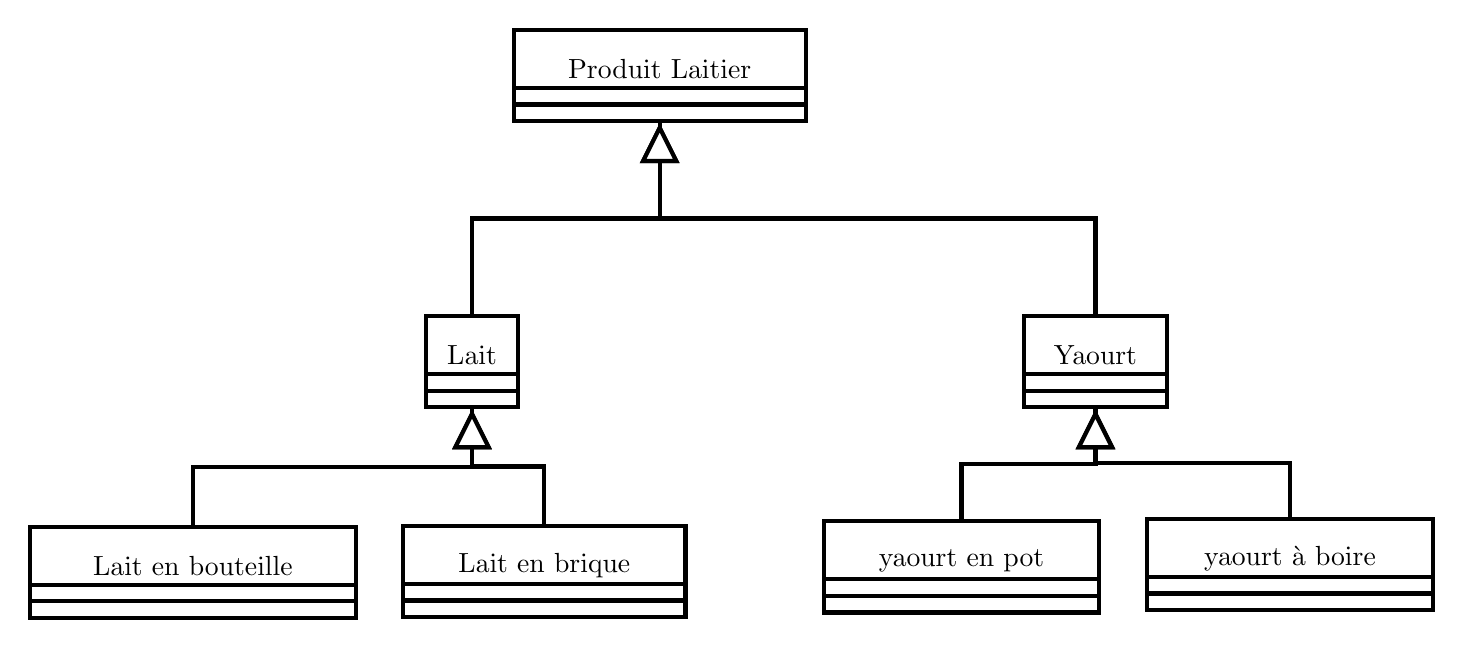
\begin{tikzpicture}
\pgftransformxscale{1.000000}
\pgftransformyscale{-1.000000}
\definecolor{dialinecolor}{rgb}{0.000000, 0.000000, 0.000000}
\pgfsetstrokecolor{dialinecolor}
\definecolor{dialinecolor}{rgb}{1.000000, 1.000000, 1.000000}
\pgfsetfillcolor{dialinecolor}
\pgfsetlinewidth{0.100000\du}
\pgfsetdash{}{0pt}
\definecolor{dialinecolor}{rgb}{1.000000, 1.000000, 1.000000}
\pgfsetfillcolor{dialinecolor}
\fill (16.775000\du,-1.635000\du)--(16.775000\du,-0.235000\du)--(23.805000\du,-0.235000\du)--(23.805000\du,-1.635000\du)--cycle;
\definecolor{dialinecolor}{rgb}{0.000000, 0.000000, 0.000000}
\pgfsetstrokecolor{dialinecolor}
\draw (16.775000\du,-1.635000\du)--(16.775000\du,-0.235000\du)--(23.805000\du,-0.235000\du)--(23.805000\du,-1.635000\du)--cycle;
% setfont left to latex
\definecolor{dialinecolor}{rgb}{0.000000, 0.000000, 0.000000}
\pgfsetstrokecolor{dialinecolor}
\node at (20.290000\du,-0.685000\du){Produit Laitier};
\definecolor{dialinecolor}{rgb}{1.000000, 1.000000, 1.000000}
\pgfsetfillcolor{dialinecolor}
\fill (16.775000\du,-0.235000\du)--(16.775000\du,0.165000\du)--(23.805000\du,0.165000\du)--(23.805000\du,-0.235000\du)--cycle;
\definecolor{dialinecolor}{rgb}{0.000000, 0.000000, 0.000000}
\pgfsetstrokecolor{dialinecolor}
\draw (16.775000\du,-0.235000\du)--(16.775000\du,0.165000\du)--(23.805000\du,0.165000\du)--(23.805000\du,-0.235000\du)--cycle;
\definecolor{dialinecolor}{rgb}{1.000000, 1.000000, 1.000000}
\pgfsetfillcolor{dialinecolor}
\fill (16.775000\du,0.165000\du)--(16.775000\du,0.565000\du)--(23.805000\du,0.565000\du)--(23.805000\du,0.165000\du)--cycle;
\definecolor{dialinecolor}{rgb}{0.000000, 0.000000, 0.000000}
\pgfsetstrokecolor{dialinecolor}
\draw (16.775000\du,0.165000\du)--(16.775000\du,0.565000\du)--(23.805000\du,0.565000\du)--(23.805000\du,0.165000\du)--cycle;
\pgfsetlinewidth{0.100000\du}
\pgfsetdash{}{0pt}
\definecolor{dialinecolor}{rgb}{1.000000, 1.000000, 1.000000}
\pgfsetfillcolor{dialinecolor}
\fill (14.665000\du,5.260000\du)--(14.665000\du,6.660000\du)--(16.872500\du,6.660000\du)--(16.872500\du,5.260000\du)--cycle;
\definecolor{dialinecolor}{rgb}{0.000000, 0.000000, 0.000000}
\pgfsetstrokecolor{dialinecolor}
\draw (14.665000\du,5.260000\du)--(14.665000\du,6.660000\du)--(16.872500\du,6.660000\du)--(16.872500\du,5.260000\du)--cycle;
% setfont left to latex
\definecolor{dialinecolor}{rgb}{0.000000, 0.000000, 0.000000}
\pgfsetstrokecolor{dialinecolor}
\node at (15.768750\du,6.210000\du){Lait};
\definecolor{dialinecolor}{rgb}{1.000000, 1.000000, 1.000000}
\pgfsetfillcolor{dialinecolor}
\fill (14.665000\du,6.660000\du)--(14.665000\du,7.060000\du)--(16.872500\du,7.060000\du)--(16.872500\du,6.660000\du)--cycle;
\definecolor{dialinecolor}{rgb}{0.000000, 0.000000, 0.000000}
\pgfsetstrokecolor{dialinecolor}
\draw (14.665000\du,6.660000\du)--(14.665000\du,7.060000\du)--(16.872500\du,7.060000\du)--(16.872500\du,6.660000\du)--cycle;
\definecolor{dialinecolor}{rgb}{1.000000, 1.000000, 1.000000}
\pgfsetfillcolor{dialinecolor}
\fill (14.665000\du,7.060000\du)--(14.665000\du,7.460000\du)--(16.872500\du,7.460000\du)--(16.872500\du,7.060000\du)--cycle;
\definecolor{dialinecolor}{rgb}{0.000000, 0.000000, 0.000000}
\pgfsetstrokecolor{dialinecolor}
\draw (14.665000\du,7.060000\du)--(14.665000\du,7.460000\du)--(16.872500\du,7.460000\du)--(16.872500\du,7.060000\du)--cycle;
\pgfsetlinewidth{0.100000\du}
\pgfsetdash{}{0pt}
\definecolor{dialinecolor}{rgb}{1.000000, 1.000000, 1.000000}
\pgfsetfillcolor{dialinecolor}
\fill (29.065000\du,5.260000\du)--(29.065000\du,6.660000\du)--(32.510000\du,6.660000\du)--(32.510000\du,5.260000\du)--cycle;
\definecolor{dialinecolor}{rgb}{0.000000, 0.000000, 0.000000}
\pgfsetstrokecolor{dialinecolor}
\draw (29.065000\du,5.260000\du)--(29.065000\du,6.660000\du)--(32.510000\du,6.660000\du)--(32.510000\du,5.260000\du)--cycle;
% setfont left to latex
\definecolor{dialinecolor}{rgb}{0.000000, 0.000000, 0.000000}
\pgfsetstrokecolor{dialinecolor}
\node at (30.787500\du,6.210000\du){Yaourt};
\definecolor{dialinecolor}{rgb}{1.000000, 1.000000, 1.000000}
\pgfsetfillcolor{dialinecolor}
\fill (29.065000\du,6.660000\du)--(29.065000\du,7.060000\du)--(32.510000\du,7.060000\du)--(32.510000\du,6.660000\du)--cycle;
\definecolor{dialinecolor}{rgb}{0.000000, 0.000000, 0.000000}
\pgfsetstrokecolor{dialinecolor}
\draw (29.065000\du,6.660000\du)--(29.065000\du,7.060000\du)--(32.510000\du,7.060000\du)--(32.510000\du,6.660000\du)--cycle;
\definecolor{dialinecolor}{rgb}{1.000000, 1.000000, 1.000000}
\pgfsetfillcolor{dialinecolor}
\fill (29.065000\du,7.060000\du)--(29.065000\du,7.460000\du)--(32.510000\du,7.460000\du)--(32.510000\du,7.060000\du)--cycle;
\definecolor{dialinecolor}{rgb}{0.000000, 0.000000, 0.000000}
\pgfsetstrokecolor{dialinecolor}
\draw (29.065000\du,7.060000\du)--(29.065000\du,7.460000\du)--(32.510000\du,7.460000\du)--(32.510000\du,7.060000\du)--cycle;
\pgfsetlinewidth{0.100000\du}
\pgfsetdash{}{0pt}
\pgfsetmiterjoin
\pgfsetbuttcap
{
\definecolor{dialinecolor}{rgb}{0.000000, 0.000000, 0.000000}
\pgfsetfillcolor{dialinecolor}
% was here!!!
\definecolor{dialinecolor}{rgb}{0.000000, 0.000000, 0.000000}
\pgfsetstrokecolor{dialinecolor}
\draw (20.290000\du,0.615281\du)--(20.290000\du,2.912500\du)--(15.768750\du,2.912500\du)--(15.768750\du,5.209719\du);
}
\definecolor{dialinecolor}{rgb}{0.000000, 0.000000, 0.000000}
\pgfsetstrokecolor{dialinecolor}
\draw (20.290000\du,1.527084\du)--(20.290000\du,2.912500\du)--(15.768750\du,2.912500\du)--(15.768750\du,5.209719\du);
\pgfsetmiterjoin
\definecolor{dialinecolor}{rgb}{1.000000, 1.000000, 1.000000}
\pgfsetfillcolor{dialinecolor}
\fill (20.690000\du,1.527084\du)--(20.290000\du,0.727084\du)--(19.890000\du,1.527084\du)--cycle;
\pgfsetlinewidth{0.100000\du}
\pgfsetdash{}{0pt}
\pgfsetmiterjoin
\definecolor{dialinecolor}{rgb}{0.000000, 0.000000, 0.000000}
\pgfsetstrokecolor{dialinecolor}
\draw (20.690000\du,1.527084\du)--(20.290000\du,0.727084\du)--(19.890000\du,1.527084\du)--cycle;
% setfont left to latex
\pgfsetlinewidth{0.100000\du}
\pgfsetdash{}{0pt}
\pgfsetmiterjoin
\pgfsetbuttcap
{
\definecolor{dialinecolor}{rgb}{0.000000, 0.000000, 0.000000}
\pgfsetfillcolor{dialinecolor}
% was here!!!
\definecolor{dialinecolor}{rgb}{0.000000, 0.000000, 0.000000}
\pgfsetstrokecolor{dialinecolor}
\draw (20.290000\du,0.615281\du)--(20.290000\du,2.912500\du)--(30.787500\du,2.912500\du)--(30.787500\du,5.209719\du);
}
\definecolor{dialinecolor}{rgb}{0.000000, 0.000000, 0.000000}
\pgfsetstrokecolor{dialinecolor}
\draw (20.290000\du,1.527084\du)--(20.290000\du,2.912500\du)--(30.787500\du,2.912500\du)--(30.787500\du,5.209719\du);
\pgfsetmiterjoin
\definecolor{dialinecolor}{rgb}{1.000000, 1.000000, 1.000000}
\pgfsetfillcolor{dialinecolor}
\fill (20.690000\du,1.527084\du)--(20.290000\du,0.727084\du)--(19.890000\du,1.527084\du)--cycle;
\pgfsetlinewidth{0.100000\du}
\pgfsetdash{}{0pt}
\pgfsetmiterjoin
\definecolor{dialinecolor}{rgb}{0.000000, 0.000000, 0.000000}
\pgfsetstrokecolor{dialinecolor}
\draw (20.690000\du,1.527084\du)--(20.290000\du,0.727084\du)--(19.890000\du,1.527084\du)--cycle;
% setfont left to latex
\pgfsetlinewidth{0.100000\du}
\pgfsetdash{}{0pt}
\definecolor{dialinecolor}{rgb}{1.000000, 1.000000, 1.000000}
\pgfsetfillcolor{dialinecolor}
\fill (5.115000\du,10.335000\du)--(5.115000\du,11.735000\du)--(12.975000\du,11.735000\du)--(12.975000\du,10.335000\du)--cycle;
\definecolor{dialinecolor}{rgb}{0.000000, 0.000000, 0.000000}
\pgfsetstrokecolor{dialinecolor}
\draw (5.115000\du,10.335000\du)--(5.115000\du,11.735000\du)--(12.975000\du,11.735000\du)--(12.975000\du,10.335000\du)--cycle;
% setfont left to latex
\definecolor{dialinecolor}{rgb}{0.000000, 0.000000, 0.000000}
\pgfsetstrokecolor{dialinecolor}
\node at (9.045000\du,11.285000\du){Lait en bouteille};
\definecolor{dialinecolor}{rgb}{1.000000, 1.000000, 1.000000}
\pgfsetfillcolor{dialinecolor}
\fill (5.115000\du,11.735000\du)--(5.115000\du,12.135000\du)--(12.975000\du,12.135000\du)--(12.975000\du,11.735000\du)--cycle;
\definecolor{dialinecolor}{rgb}{0.000000, 0.000000, 0.000000}
\pgfsetstrokecolor{dialinecolor}
\draw (5.115000\du,11.735000\du)--(5.115000\du,12.135000\du)--(12.975000\du,12.135000\du)--(12.975000\du,11.735000\du)--cycle;
\definecolor{dialinecolor}{rgb}{1.000000, 1.000000, 1.000000}
\pgfsetfillcolor{dialinecolor}
\fill (5.115000\du,12.135000\du)--(5.115000\du,12.535000\du)--(12.975000\du,12.535000\du)--(12.975000\du,12.135000\du)--cycle;
\definecolor{dialinecolor}{rgb}{0.000000, 0.000000, 0.000000}
\pgfsetstrokecolor{dialinecolor}
\draw (5.115000\du,12.135000\du)--(5.115000\du,12.535000\du)--(12.975000\du,12.535000\du)--(12.975000\du,12.135000\du)--cycle;
\pgfsetlinewidth{0.100000\du}
\pgfsetdash{}{0pt}
\definecolor{dialinecolor}{rgb}{1.000000, 1.000000, 1.000000}
\pgfsetfillcolor{dialinecolor}
\fill (32.030000\du,10.145000\du)--(32.030000\du,11.545000\du)--(38.920000\du,11.545000\du)--(38.920000\du,10.145000\du)--cycle;
\definecolor{dialinecolor}{rgb}{0.000000, 0.000000, 0.000000}
\pgfsetstrokecolor{dialinecolor}
\draw (32.030000\du,10.145000\du)--(32.030000\du,11.545000\du)--(38.920000\du,11.545000\du)--(38.920000\du,10.145000\du)--cycle;
% setfont left to latex
\definecolor{dialinecolor}{rgb}{0.000000, 0.000000, 0.000000}
\pgfsetstrokecolor{dialinecolor}
\node at (35.475000\du,11.095000\du){yaourt à boire};
\definecolor{dialinecolor}{rgb}{1.000000, 1.000000, 1.000000}
\pgfsetfillcolor{dialinecolor}
\fill (32.030000\du,11.545000\du)--(32.030000\du,11.945000\du)--(38.920000\du,11.945000\du)--(38.920000\du,11.545000\du)--cycle;
\definecolor{dialinecolor}{rgb}{0.000000, 0.000000, 0.000000}
\pgfsetstrokecolor{dialinecolor}
\draw (32.030000\du,11.545000\du)--(32.030000\du,11.945000\du)--(38.920000\du,11.945000\du)--(38.920000\du,11.545000\du)--cycle;
\definecolor{dialinecolor}{rgb}{1.000000, 1.000000, 1.000000}
\pgfsetfillcolor{dialinecolor}
\fill (32.030000\du,11.945000\du)--(32.030000\du,12.345000\du)--(38.920000\du,12.345000\du)--(38.920000\du,11.945000\du)--cycle;
\definecolor{dialinecolor}{rgb}{0.000000, 0.000000, 0.000000}
\pgfsetstrokecolor{dialinecolor}
\draw (32.030000\du,11.945000\du)--(32.030000\du,12.345000\du)--(38.920000\du,12.345000\du)--(38.920000\du,11.945000\du)--cycle;
\pgfsetlinewidth{0.100000\du}
\pgfsetdash{}{0pt}
\definecolor{dialinecolor}{rgb}{1.000000, 1.000000, 1.000000}
\pgfsetfillcolor{dialinecolor}
\fill (24.245000\du,10.205000\du)--(24.245000\du,11.605000\du)--(30.877500\du,11.605000\du)--(30.877500\du,10.205000\du)--cycle;
\definecolor{dialinecolor}{rgb}{0.000000, 0.000000, 0.000000}
\pgfsetstrokecolor{dialinecolor}
\draw (24.245000\du,10.205000\du)--(24.245000\du,11.605000\du)--(30.877500\du,11.605000\du)--(30.877500\du,10.205000\du)--cycle;
% setfont left to latex
\definecolor{dialinecolor}{rgb}{0.000000, 0.000000, 0.000000}
\pgfsetstrokecolor{dialinecolor}
\node at (27.561250\du,11.155000\du){yaourt en pot};
\definecolor{dialinecolor}{rgb}{1.000000, 1.000000, 1.000000}
\pgfsetfillcolor{dialinecolor}
\fill (24.245000\du,11.605000\du)--(24.245000\du,12.005000\du)--(30.877500\du,12.005000\du)--(30.877500\du,11.605000\du)--cycle;
\definecolor{dialinecolor}{rgb}{0.000000, 0.000000, 0.000000}
\pgfsetstrokecolor{dialinecolor}
\draw (24.245000\du,11.605000\du)--(24.245000\du,12.005000\du)--(30.877500\du,12.005000\du)--(30.877500\du,11.605000\du)--cycle;
\definecolor{dialinecolor}{rgb}{1.000000, 1.000000, 1.000000}
\pgfsetfillcolor{dialinecolor}
\fill (24.245000\du,12.005000\du)--(24.245000\du,12.405000\du)--(30.877500\du,12.405000\du)--(30.877500\du,12.005000\du)--cycle;
\definecolor{dialinecolor}{rgb}{0.000000, 0.000000, 0.000000}
\pgfsetstrokecolor{dialinecolor}
\draw (24.245000\du,12.005000\du)--(24.245000\du,12.405000\du)--(30.877500\du,12.405000\du)--(30.877500\du,12.005000\du)--cycle;
\pgfsetlinewidth{0.100000\du}
\pgfsetdash{}{0pt}
\definecolor{dialinecolor}{rgb}{1.000000, 1.000000, 1.000000}
\pgfsetfillcolor{dialinecolor}
\fill (14.110000\du,10.315000\du)--(14.110000\du,11.715000\du)--(20.912500\du,11.715000\du)--(20.912500\du,10.315000\du)--cycle;
\definecolor{dialinecolor}{rgb}{0.000000, 0.000000, 0.000000}
\pgfsetstrokecolor{dialinecolor}
\draw (14.110000\du,10.315000\du)--(14.110000\du,11.715000\du)--(20.912500\du,11.715000\du)--(20.912500\du,10.315000\du)--cycle;
% setfont left to latex
\definecolor{dialinecolor}{rgb}{0.000000, 0.000000, 0.000000}
\pgfsetstrokecolor{dialinecolor}
\node at (17.511250\du,11.265000\du){Lait en brique};
\definecolor{dialinecolor}{rgb}{1.000000, 1.000000, 1.000000}
\pgfsetfillcolor{dialinecolor}
\fill (14.110000\du,11.715000\du)--(14.110000\du,12.115000\du)--(20.912500\du,12.115000\du)--(20.912500\du,11.715000\du)--cycle;
\definecolor{dialinecolor}{rgb}{0.000000, 0.000000, 0.000000}
\pgfsetstrokecolor{dialinecolor}
\draw (14.110000\du,11.715000\du)--(14.110000\du,12.115000\du)--(20.912500\du,12.115000\du)--(20.912500\du,11.715000\du)--cycle;
\definecolor{dialinecolor}{rgb}{1.000000, 1.000000, 1.000000}
\pgfsetfillcolor{dialinecolor}
\fill (14.110000\du,12.115000\du)--(14.110000\du,12.515000\du)--(20.912500\du,12.515000\du)--(20.912500\du,12.115000\du)--cycle;
\definecolor{dialinecolor}{rgb}{0.000000, 0.000000, 0.000000}
\pgfsetstrokecolor{dialinecolor}
\draw (14.110000\du,12.115000\du)--(14.110000\du,12.515000\du)--(20.912500\du,12.515000\du)--(20.912500\du,12.115000\du)--cycle;
\pgfsetlinewidth{0.100000\du}
\pgfsetdash{}{0pt}
\pgfsetmiterjoin
\pgfsetbuttcap
{
\definecolor{dialinecolor}{rgb}{0.000000, 0.000000, 0.000000}
\pgfsetfillcolor{dialinecolor}
% was here!!!
\definecolor{dialinecolor}{rgb}{0.000000, 0.000000, 0.000000}
\pgfsetstrokecolor{dialinecolor}
\draw (15.768750\du,7.510281\du)--(15.768750\du,8.897500\du)--(9.045000\du,8.897500\du)--(9.045000\du,10.284719\du);
}
\definecolor{dialinecolor}{rgb}{0.000000, 0.000000, 0.000000}
\pgfsetstrokecolor{dialinecolor}
\draw (15.768750\du,8.422084\du)--(15.768750\du,8.897500\du)--(9.045000\du,8.897500\du)--(9.045000\du,10.284719\du);
\pgfsetmiterjoin
\definecolor{dialinecolor}{rgb}{1.000000, 1.000000, 1.000000}
\pgfsetfillcolor{dialinecolor}
\fill (16.168750\du,8.422084\du)--(15.768750\du,7.622084\du)--(15.368750\du,8.422084\du)--cycle;
\pgfsetlinewidth{0.100000\du}
\pgfsetdash{}{0pt}
\pgfsetmiterjoin
\definecolor{dialinecolor}{rgb}{0.000000, 0.000000, 0.000000}
\pgfsetstrokecolor{dialinecolor}
\draw (16.168750\du,8.422084\du)--(15.768750\du,7.622084\du)--(15.368750\du,8.422084\du)--cycle;
% setfont left to latex
\pgfsetlinewidth{0.100000\du}
\pgfsetdash{}{0pt}
\pgfsetmiterjoin
\pgfsetbuttcap
{
\definecolor{dialinecolor}{rgb}{0.000000, 0.000000, 0.000000}
\pgfsetfillcolor{dialinecolor}
% was here!!!
\definecolor{dialinecolor}{rgb}{0.000000, 0.000000, 0.000000}
\pgfsetstrokecolor{dialinecolor}
\draw (15.768750\du,7.510281\du)--(15.768750\du,8.887500\du)--(17.511250\du,8.887500\du)--(17.511250\du,10.264719\du);
}
\definecolor{dialinecolor}{rgb}{0.000000, 0.000000, 0.000000}
\pgfsetstrokecolor{dialinecolor}
\draw (15.768750\du,8.422084\du)--(15.768750\du,8.887500\du)--(17.511250\du,8.887500\du)--(17.511250\du,10.264719\du);
\pgfsetmiterjoin
\definecolor{dialinecolor}{rgb}{1.000000, 1.000000, 1.000000}
\pgfsetfillcolor{dialinecolor}
\fill (16.168750\du,8.422084\du)--(15.768750\du,7.622084\du)--(15.368750\du,8.422084\du)--cycle;
\pgfsetlinewidth{0.100000\du}
\pgfsetdash{}{0pt}
\pgfsetmiterjoin
\definecolor{dialinecolor}{rgb}{0.000000, 0.000000, 0.000000}
\pgfsetstrokecolor{dialinecolor}
\draw (16.168750\du,8.422084\du)--(15.768750\du,7.622084\du)--(15.368750\du,8.422084\du)--cycle;
% setfont left to latex
\pgfsetlinewidth{0.100000\du}
\pgfsetdash{}{0pt}
\pgfsetmiterjoin
\pgfsetbuttcap
{
\definecolor{dialinecolor}{rgb}{0.000000, 0.000000, 0.000000}
\pgfsetfillcolor{dialinecolor}
% was here!!!
\definecolor{dialinecolor}{rgb}{0.000000, 0.000000, 0.000000}
\pgfsetstrokecolor{dialinecolor}
\draw (30.787500\du,7.510281\du)--(30.787500\du,8.832500\du)--(27.561250\du,8.832500\du)--(27.561250\du,10.154719\du);
}
\definecolor{dialinecolor}{rgb}{0.000000, 0.000000, 0.000000}
\pgfsetstrokecolor{dialinecolor}
\draw (30.787500\du,8.422084\du)--(30.787500\du,8.832500\du)--(27.561250\du,8.832500\du)--(27.561250\du,10.154719\du);
\pgfsetmiterjoin
\definecolor{dialinecolor}{rgb}{1.000000, 1.000000, 1.000000}
\pgfsetfillcolor{dialinecolor}
\fill (31.187500\du,8.422084\du)--(30.787500\du,7.622084\du)--(30.387500\du,8.422084\du)--cycle;
\pgfsetlinewidth{0.100000\du}
\pgfsetdash{}{0pt}
\pgfsetmiterjoin
\definecolor{dialinecolor}{rgb}{0.000000, 0.000000, 0.000000}
\pgfsetstrokecolor{dialinecolor}
\draw (31.187500\du,8.422084\du)--(30.787500\du,7.622084\du)--(30.387500\du,8.422084\du)--cycle;
% setfont left to latex
\pgfsetlinewidth{0.100000\du}
\pgfsetdash{}{0pt}
\pgfsetmiterjoin
\pgfsetbuttcap
{
\definecolor{dialinecolor}{rgb}{0.000000, 0.000000, 0.000000}
\pgfsetfillcolor{dialinecolor}
% was here!!!
\definecolor{dialinecolor}{rgb}{0.000000, 0.000000, 0.000000}
\pgfsetstrokecolor{dialinecolor}
\draw (30.787500\du,7.510281\du)--(30.787500\du,8.802500\du)--(35.475000\du,8.802500\du)--(35.475000\du,10.094719\du);
}
\definecolor{dialinecolor}{rgb}{0.000000, 0.000000, 0.000000}
\pgfsetstrokecolor{dialinecolor}
\draw (30.787500\du,8.422084\du)--(30.787500\du,8.802500\du)--(35.475000\du,8.802500\du)--(35.475000\du,10.094719\du);
\pgfsetmiterjoin
\definecolor{dialinecolor}{rgb}{1.000000, 1.000000, 1.000000}
\pgfsetfillcolor{dialinecolor}
\fill (31.187500\du,8.422084\du)--(30.787500\du,7.622084\du)--(30.387500\du,8.422084\du)--cycle;
\pgfsetlinewidth{0.100000\du}
\pgfsetdash{}{0pt}
\pgfsetmiterjoin
\definecolor{dialinecolor}{rgb}{0.000000, 0.000000, 0.000000}
\pgfsetstrokecolor{dialinecolor}
\draw (31.187500\du,8.422084\du)--(30.787500\du,7.622084\du)--(30.387500\du,8.422084\du)--cycle;
% setfont left to latex
\end{tikzpicture}
